


\documentclass{beamer}
\usetheme{ucl}

\usepackage[utf8]{inputenc}


%%% Increase the height of the banner: the argument is a scale factor >=1.0
%\setbeamertemplate{banner}[ucl][10.0]

%%% Change the colour of the main banner
%%% The background should be one of the UCL colours (except pink or white):
%%%   black,darkpurple,darkred,darkblue,darkgreen,darkbrown,richred,midred,
%%%   navyblue,midgreen,darkgrey,orange,brightblue,brightgreen,lightgrey,
%%%   lightpurple,yellow,lightblue,lightgreen,stone
\setbeamercolor{banner}{bg=darkpurple}
%\setbeamercolor{banner}{bg=yellow,fg=black}

%%% Add a stripe behind the banner
%\setbeamercolor{banner stripe}{bg=darkpurple,fg=black}

%%% The main structural elements
\setbeamercolor{structure}{fg=black}

%%% Author/Title/Date and slide number in the footline
\setbeamertemplate{footline}[author title date]

%%% Puts the section/subsection in the headline
% \setbeamertemplate{headline}[section]

%%% Puts a navigation bar on top of the banner
%%% For this to work correctly, the each \section command needs to be
%%% followed by a \subsection. Requires one extra compile.
% \setbeamertemplate{headline}[miniframes]
%%% Accepts an optional argument determining the width
% \setbeamertemplate{headline}[miniframes][0.3\paperwidth]


%%% Puts the frame title in the banner
%%% Won't work correctly with the above headline templates
%\useoutertheme{ucltitlebanner}
%%% Similar to above, but smaller (and puts subtitle on same line as title)
\useoutertheme[small]{ucltitlebanner}

%%% Gives block elements (theorems, examples) a border
% \useinnertheme{blockborder}
%%% Sets the body of block elements to be clear
% \setbeamercolor{block body}{bg=white,fg=black}

%%% Include CSML logo on title slide
%\titlegraphic{\includegraphics[width=0.16\paperwidth]{csml_logo}}

%%% Include CSML logo in bottom right corner of all slides
%\logo{\includegraphics[width=0.12\paperwidth]{csml_logo}}

%%% Set a background colour
% \setbeamercolor{background canvas}{bg=lightgrey}

%%% Set a background image
%%% Some sample images are available from the UCL image store:
%%%   https://www.imagestore.ucl.ac.uk/home/start
% \setbeamertemplate{background canvas}{%
%   \includegraphics[width=\paperwidth]{imagename}}



%%%%%% Some other settings that can make things look nicer
%%% Set a smaller indent for description environment
\setbeamersize{description width=2em}
%%% Remove nav symbols (and shift any logo down to corner)
\setbeamertemplate{navigation symbols}{\vspace{-2ex}}








\DeclareMathOperator{\Cov}{Cov}
\DeclareMathOperator{\Var}{Var}
\DeclareMathOperator{\E}{\mathbb{E}}
\DeclareMathOperator{\Proba}{\mathbb{P}}

\newcommand{\Covb}[2]{\ensuremath{\Cov\!\left[#1,#2\right]}}
\newcommand{\Eb}[1]{\ensuremath{\E\!\left[#1\right]}}
\newcommand{\Pb}[1]{\ensuremath{\Proba\!\left[#1\right]}}
\newcommand{\Varb}[1]{\ensuremath{\Var\!\left[#1\right]}}

% norm
\newcommand{\norm}[1]{\| #1 \|}

\newcommand{\indep}{\rotatebox[origin=c]{90}{$\models$}}





\usepackage{mathptmx,amsmath,amssymb,graphicx,bibentry,bbm,ragged2e}
\usepackage[english]{babel}

\makeatletter

\newcommand{\noun}[1]{\textsc{#1}}
\newcommand{\jitem}[1]{\item \begin{justify} #1 \end{justify} \vfill{}}
\newcommand{\sframe}[2]{\frame{\frametitle{#1} #2}}

\newenvironment{centercolumns}{\begin{columns}[c]}{\end{columns}}
%\newenvironment{jitem}{\begin{justify}\begin{itemize}}{\end{itemize}\end{justify}}



%\usetheme{Warsaw}
%\setbeamertemplate{footline}[text line]{}
%\setbeamertemplate{headline}{}
%\setbeamercolor{structure}{fg=purple!50!blue, bg=purple!50!blue}

%\setbeamersize{text margin left=15pt,text margin right=15pt}

%\setbeamercovered{transparent}


\@ifundefined{showcaptionsetup}{}{%
 \PassOptionsToPackage{caption=false}{subfig}}
\usepackage{subfig}

\usepackage[utf8]{inputenc}
\usepackage[T1]{fontenc}

\usepackage{multirow}


\makeatother

\def \draft {1}

\usepackage{xparse}
\usepackage{ifthen}
\DeclareDocumentCommand{\comment}{m o o o o}
{\ifthenelse{\draft=1}{
    \textcolor{red}{\textbf{C : }#1}
    \IfValueT{#2}{\textcolor{blue}{\textbf{A1 : }#2}}
    \IfValueT{#3}{\textcolor{ForestGreen}{\textbf{A2 : }#3}}
    \IfValueT{#4}{\textcolor{red!50!blue}{\textbf{A3 : }#4}}
    \IfValueT{#5}{\textcolor{Aquamarine}{\textbf{A4 : }#5}}
 }{}
}
\newcommand{\todo}[1]{
\ifthenelse{\draft=1}{\textcolor{red!50!blue}{\textbf{TODO : \textit{#1}}}}{}
}




\begin{document}


\title[HSR and access equity]{High-speed rail development and access equity: the case of Guangdong province, China}

\author[Raimbault]{Li, Zhiyuan$^1$ and Raimbault, Juste$^{1,\ast}$\\\medskip
$^{\ast}$\texttt{j.raimbault@ucl.ac.uk}
}

\institute[UCL]{$^{1}$Center for Advanced Spatial Analysis, University College London
}


\date[05/11/2021]{ECTQG 2021\\
Special Session: Sustainable Mobility and Equality in Mega-city Regions: Patterns, Mechanisms and Governance\\
November 5th 2021
}

\frame{\maketitle}


% Keywords: High-speed Rail, Access Equity, Greater Bay Area


\section{Introduction}


\sframe{High speed rail development in China}{

% In recent years, China has witnessed a nationwide and relatively fast development of high-speed rail (HSR) infrastructures, improving considerably accessibility between large cities.

Very rapid development of a new HSR network in China since 2008 (8+8 plan at the national scale) \cite{zhou2018china}

\bigskip

\begin{center}
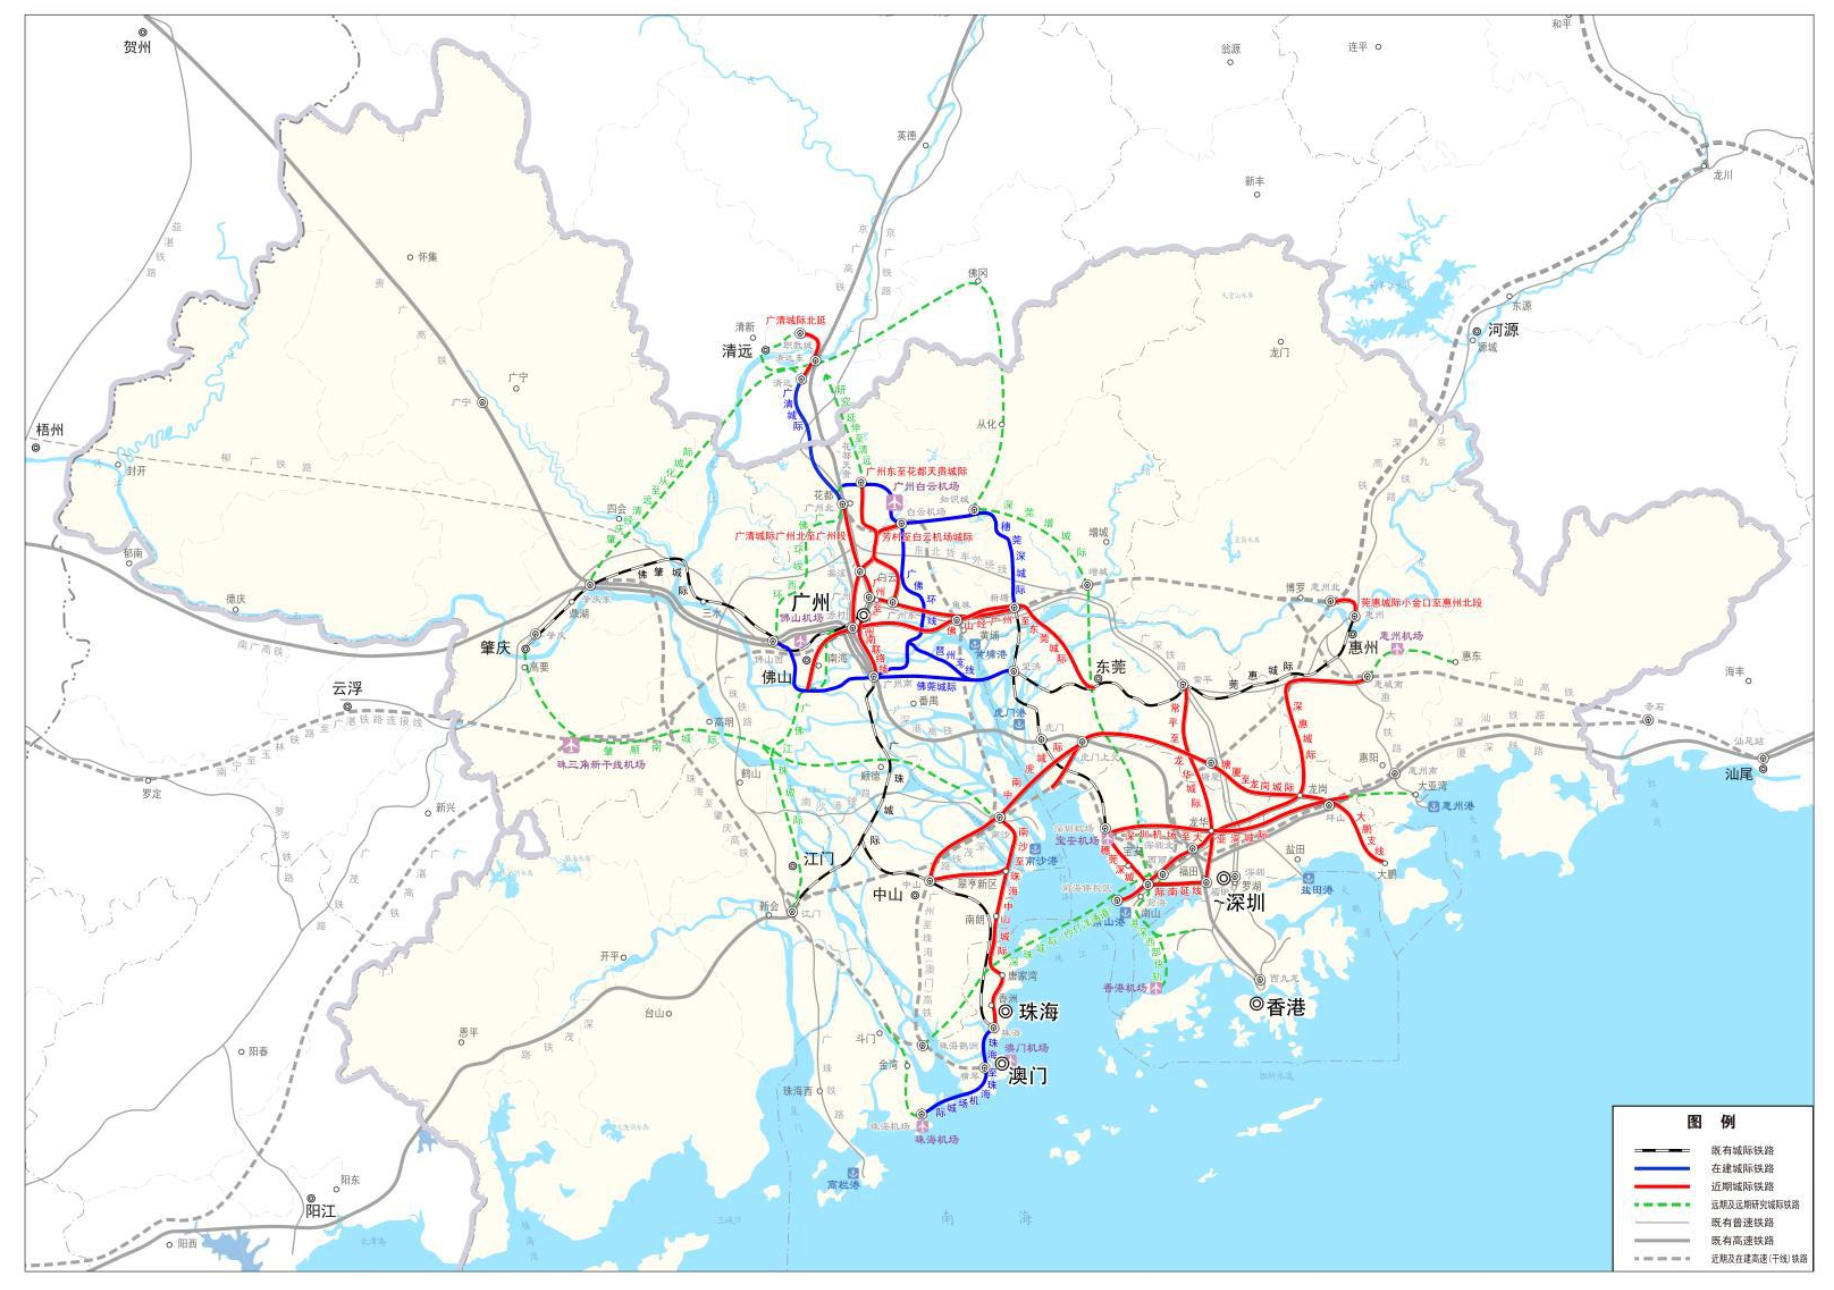
\includegraphics[width=0.6\textwidth]{figures/icr_plan.png}
\end{center}

\smallskip

\textit{Inter-city Railway plan for the Greater Bay Area (Source: China Mid-term and Long-term Railway Network Planning, 2016)}


}

\sframe{HSR and access equity}{

% At regional scales, this however implies unbalanced development, as major poles were the priority of the 8+8 planning scheme at the national scale.

Concerns over negative impact of HSR development on access equity:

\medskip

\begin{itemize}
	\item Moderate economic impact on smaller cities \cite{liu2021impacts}
	\item Increase in national accessibility inequality \cite{jiao2017impacts}
	\item Major cities negotiate station location more easily \cite{zhu2015high}
	\item Mitigation of travel time improvements due to remote stations \cite{wang2013spatial}
\end{itemize}


}

\sframe{Transport access equity}{

% In particular within mega-city regions, transport access equity becomes a central concern for future planning policies.
% defs transport equity

No unique definition of access equity \cite{kim2015impacts}:

\medskip

\begin{itemize}
	\item geographical equity \cite{welch2013equity}	
	\item socio-economic equity \cite{litman2002evaluating}
\end{itemize}

\bigskip

Methods to quantify access equity:

\medskip

\begin{itemize}
	\item Travel time improvements \cite{wang2013spatial}
	\item Generalised accessibility (opportunities) \cite{vickerman1997high}	
\end{itemize}



}

\sframe{Quantifying access equity in GBA}{

% This contribution focuses on the case of the Guangdong-Hong Kong-Macao Greater Bay Area, and more broadly on Guangdong province.

% How has HSR construction in the GBA and GD improved traffic accessibility, and what is its impact on traffic flow patterns?
%What’s HSR construction’s impact on transportation equity?
% Which cities have benefited most from the HSR construction, and which cities need enhancement?
% What is the impact of the HSR construction in the planning scenarios in the study area, not least in respect of efficiency and improved transportation equity?

Previous work on access equity in the GBA:

\begin{itemize}
	\item Access impacts in 2020 of ICR \cite{hou2011transport}
	\item Socio-economic disparities in Guangzhou \cite{chen2021socioeconomic}
	\item HSR and industrial movement \cite{chang2021high}
\end{itemize}

\bigskip

\textbf{Research question}

\medskip

\textit{What is the impact of HSR construction on accessibility and its equity; What will be the impact of mid-term and long-term planned lines?}



}


\section{Materials and methods}


\sframe{Data}{

% Gathering socio-economic data and train timetables

\begin{itemize}
	\item Road travel times scrapped from Gaode maps; train timetables gathered manually from China Railway website
	\item Tencent flow data between cities (driving, railway, plane)
	\item Socio-economic data from Guangdong statistical yearbook 2020 and HK and Macao statistics; housing prices from Anjuke website
	\item Network data (expressway and railway) from OpenStreetMap
\end{itemize}

%https://www.12306.cn/index/

\begin{center}
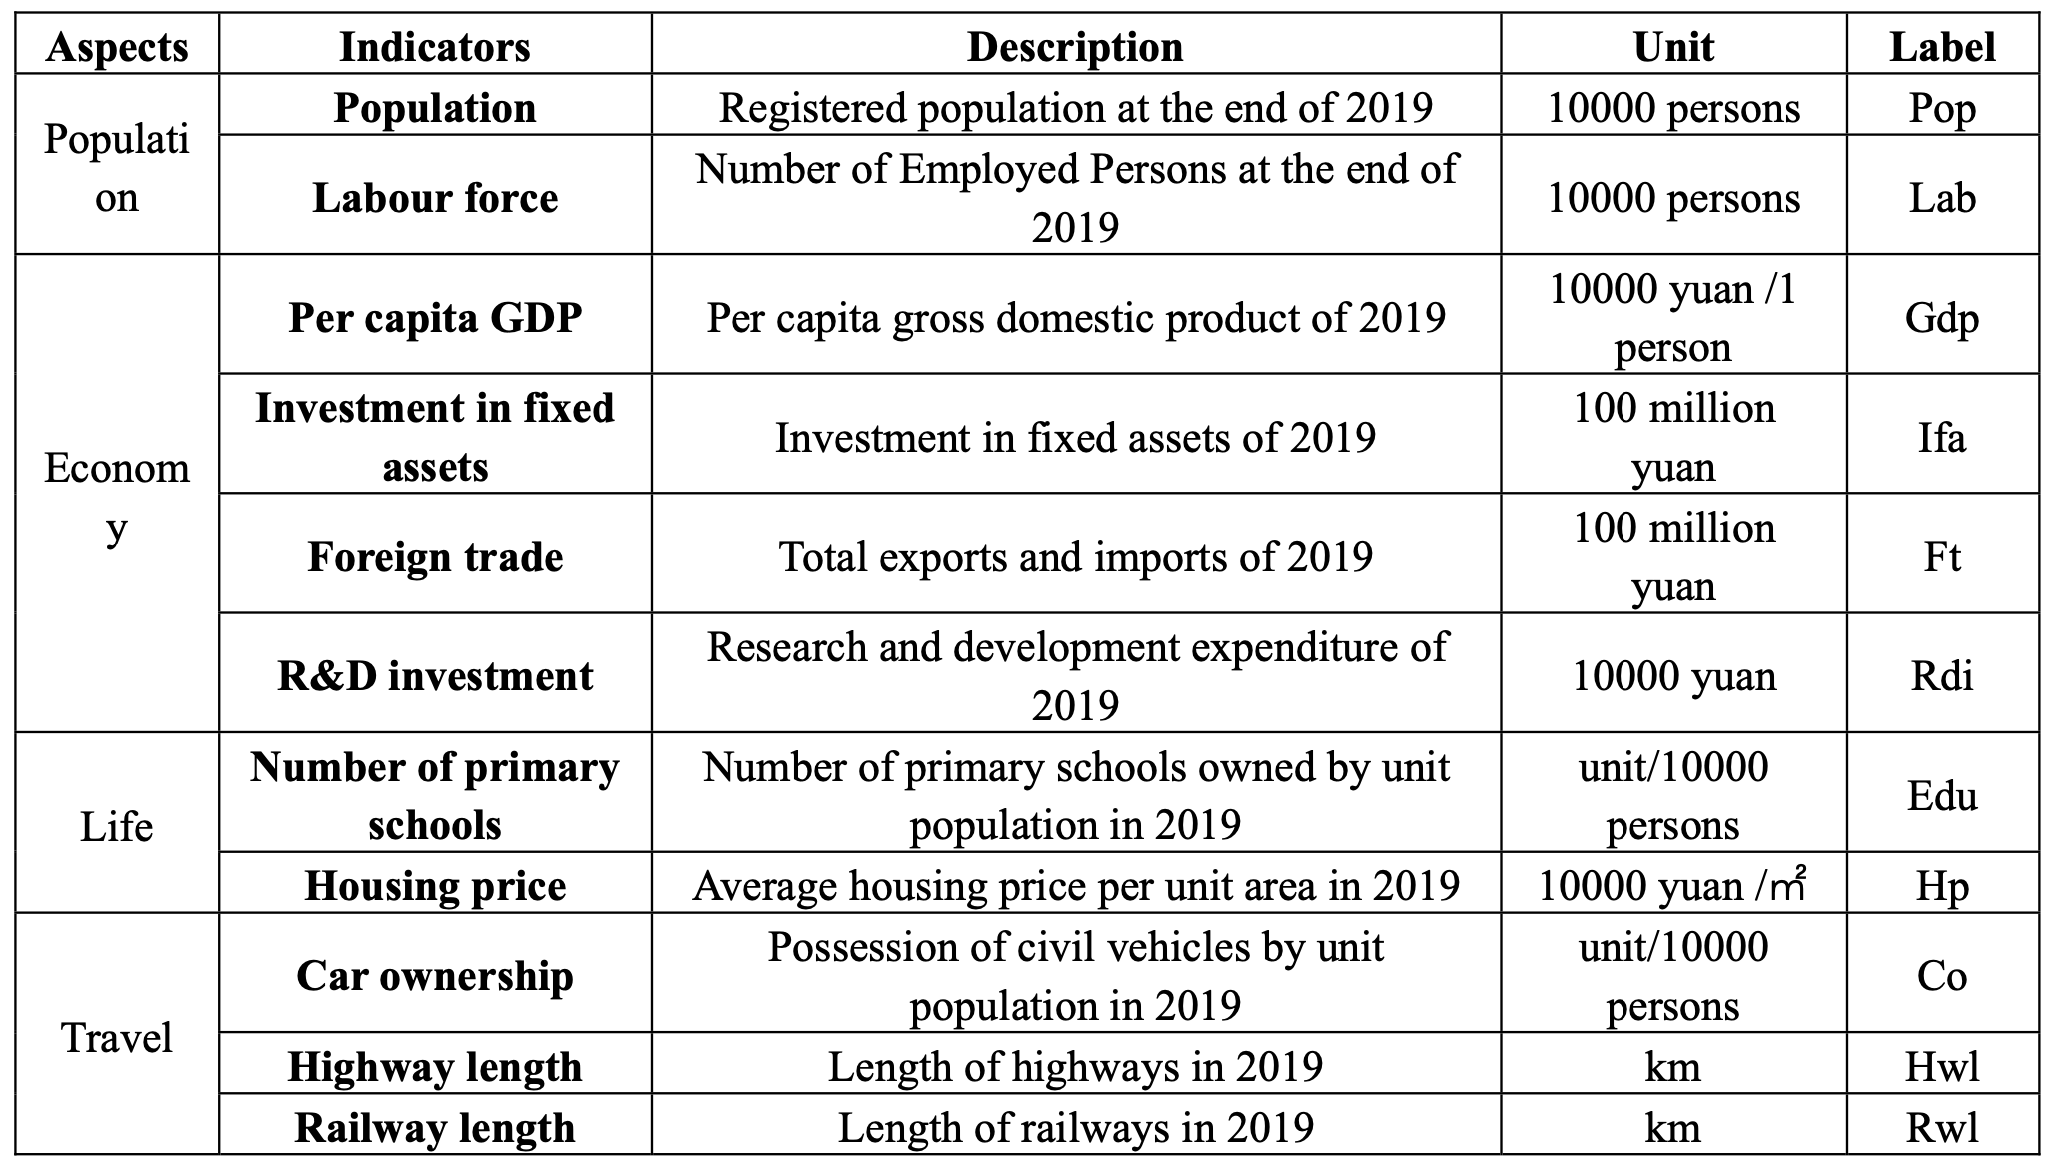
\includegraphics[width=0.5\textwidth]{figures/socioecodata.png}
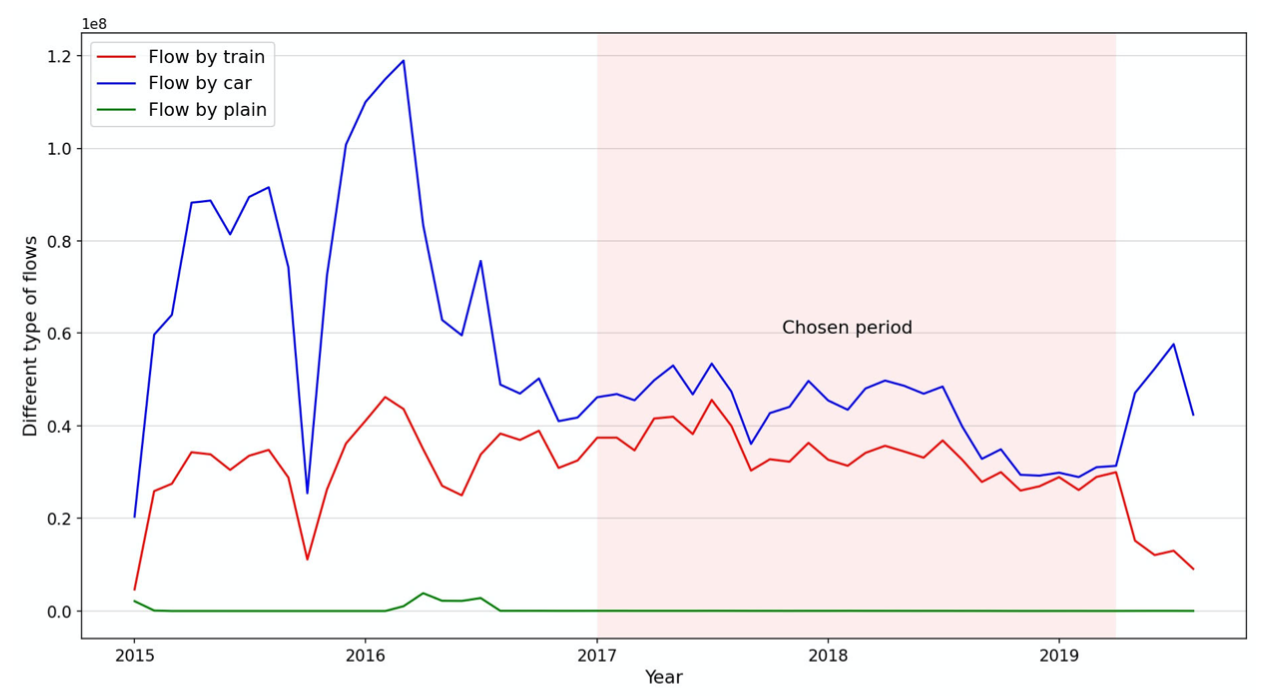
\includegraphics[width=0.5\textwidth]{figures/tencentdata.png}
\end{center}

\footnotesize
\textit{(Left) Socio-economic data for spatial interaction models; (Right) Tencent flows}

}

\sframe{Current HSR lines in the GBA}{

\centering
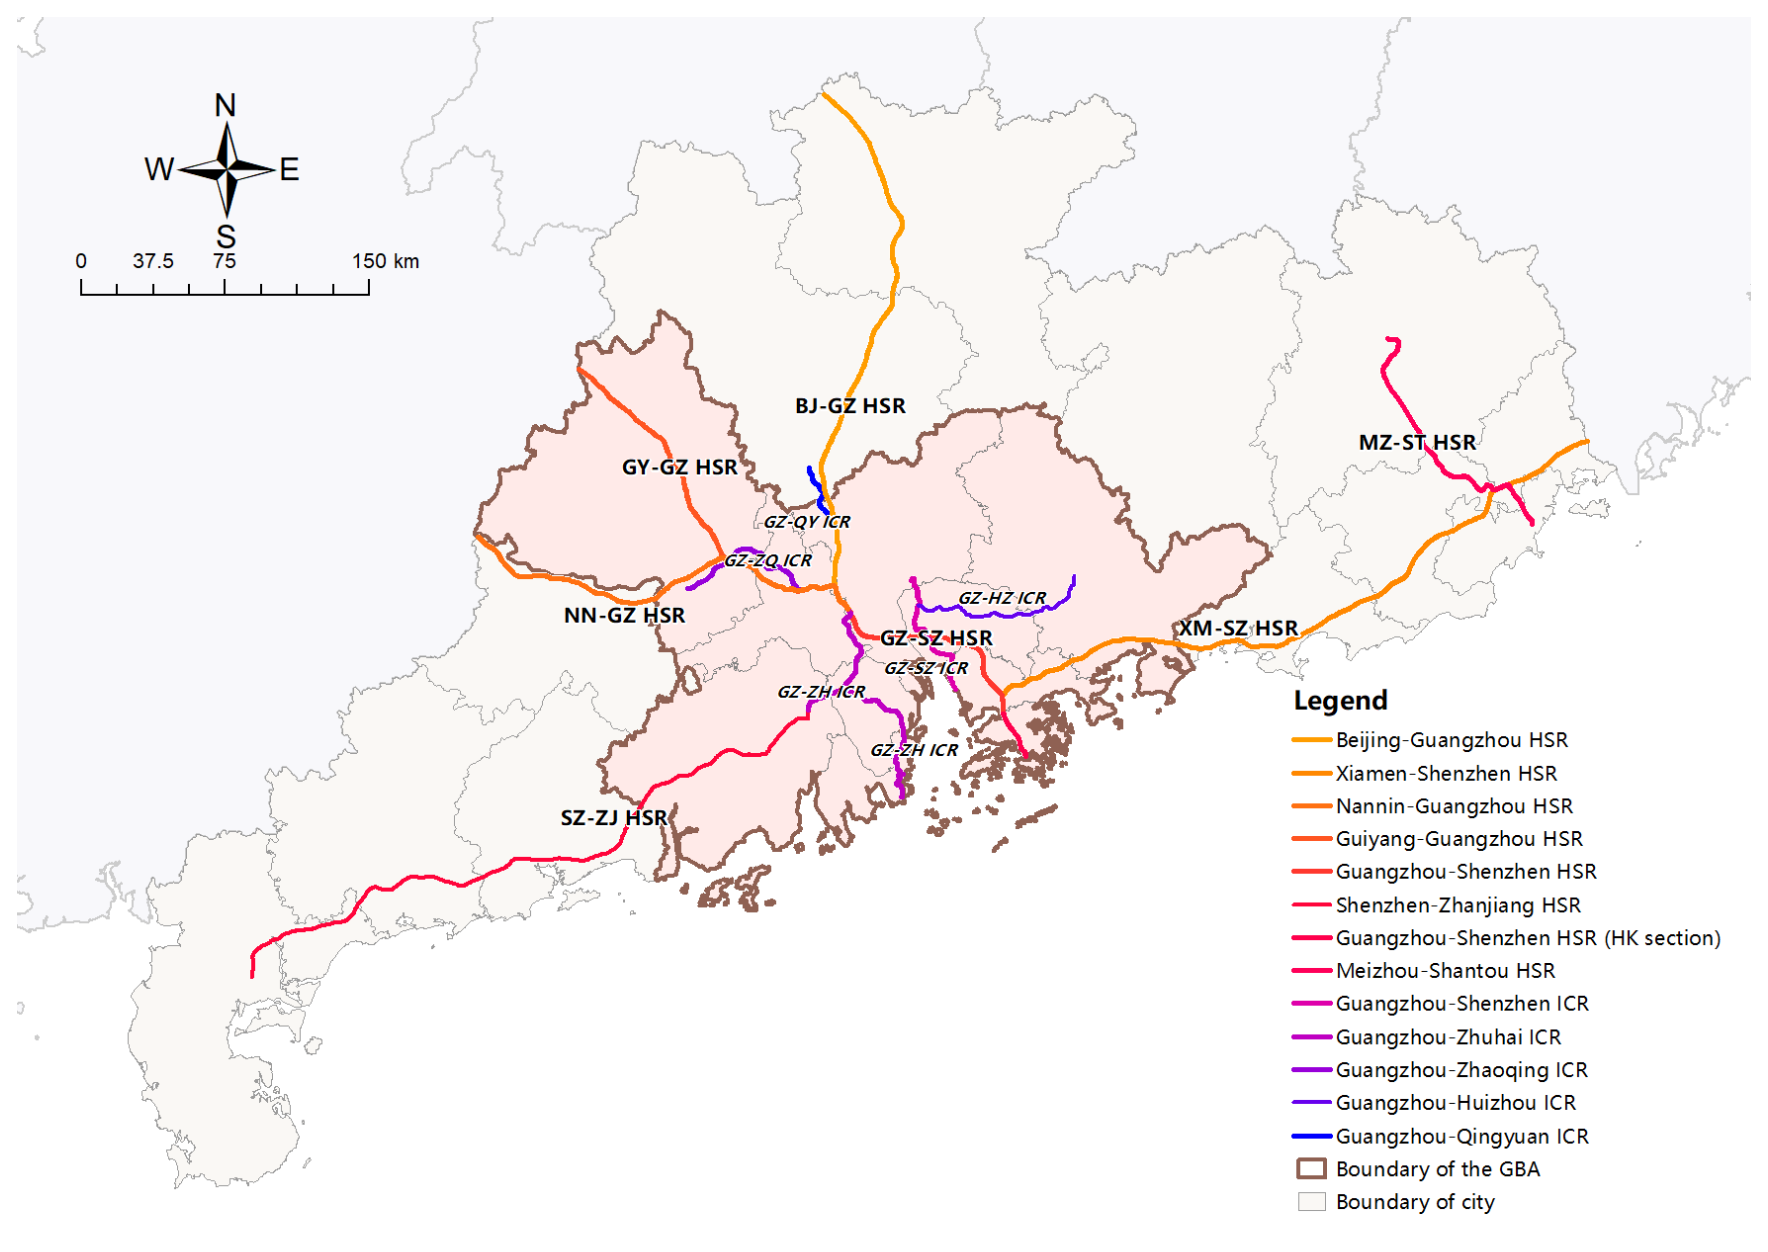
\includegraphics[width=\linewidth]{figures/current_hsr_lines.png}


}

\sframe{Planned HSR lines in the GBA}{

\centering
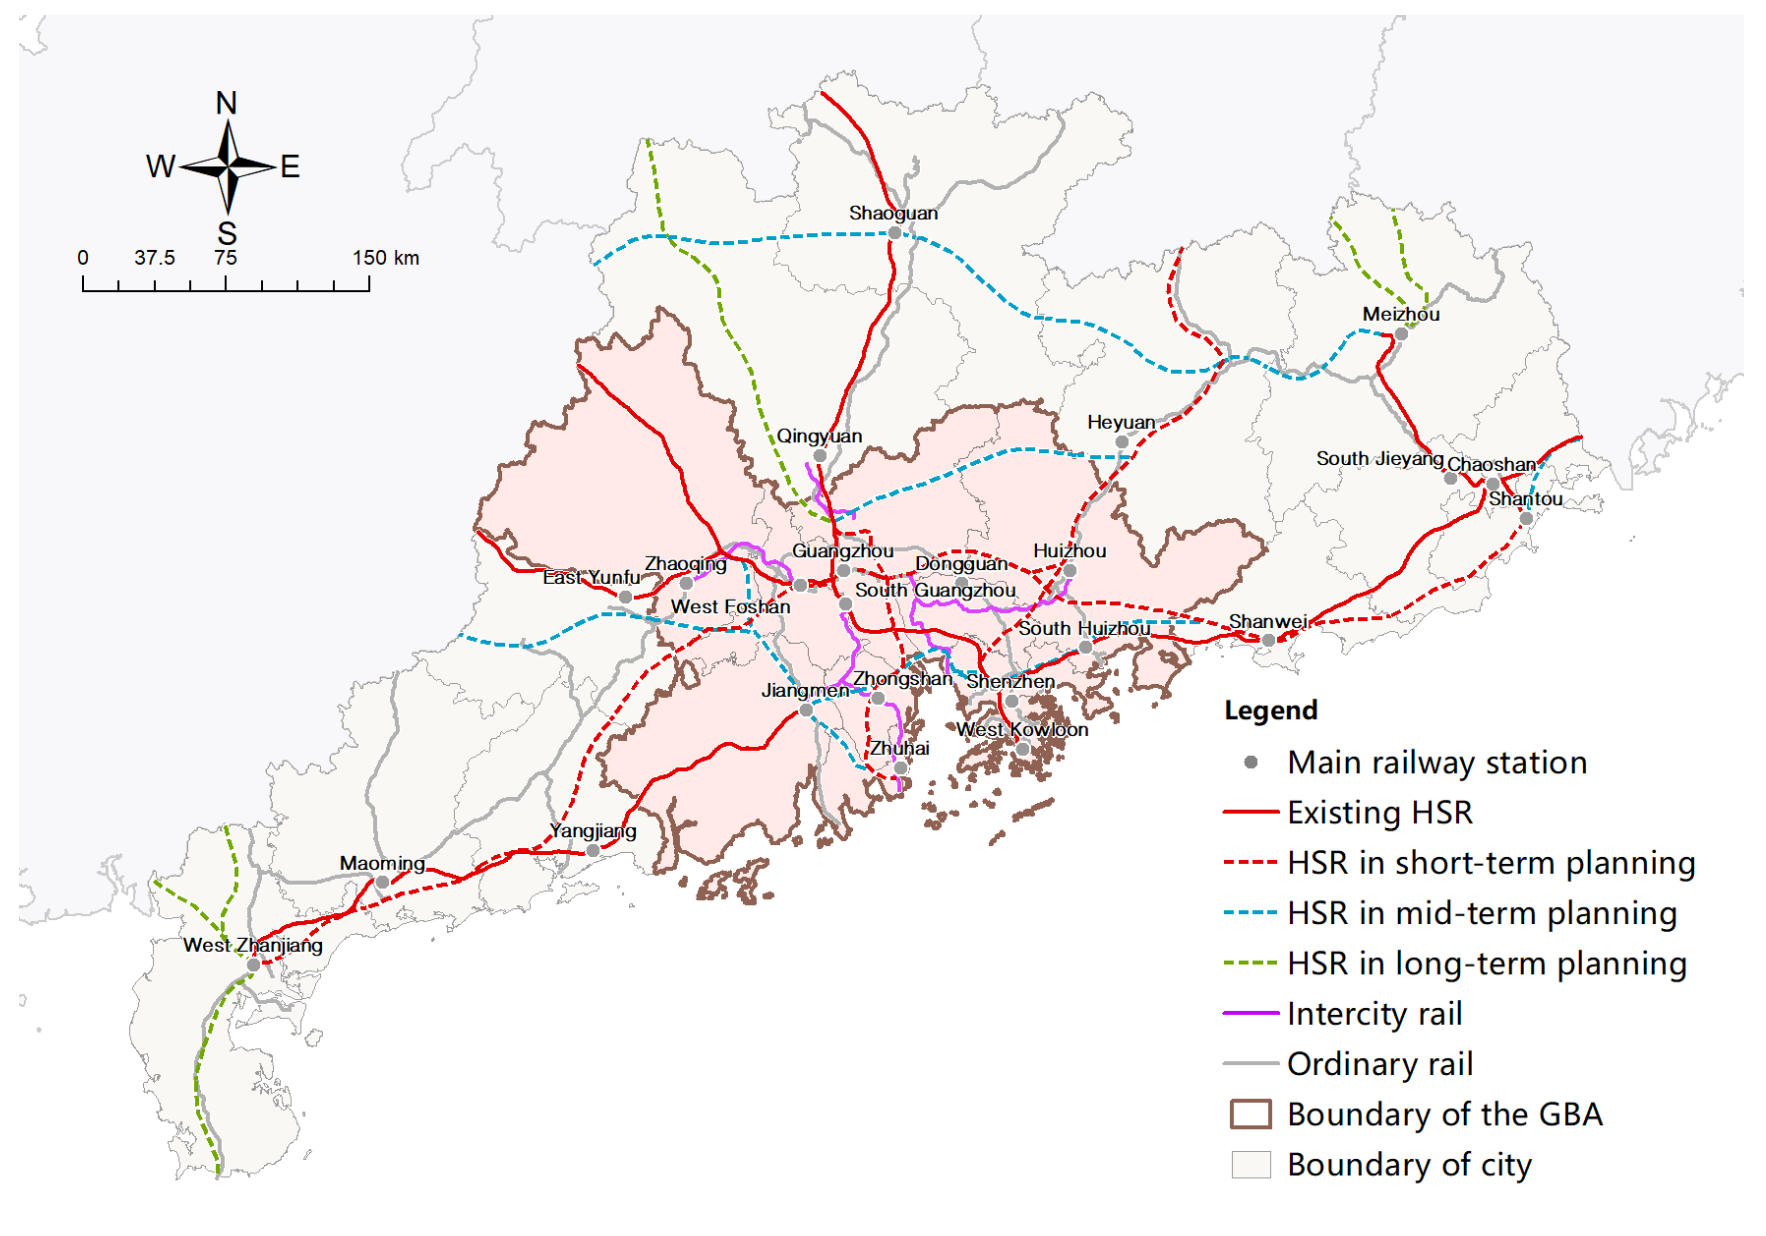
\includegraphics[width=\linewidth]{figures/planned_lines.png}

% Q: how are travel time improvement computed?-> topological data; details:?
% -> supp material (refer to github?); travel time matrices updated partly by hand?
% -> not in python, already in train table: should have been done in arcgis (rq: not totally reproducible)

}

\sframe{Methods}{

% we first build travel-time based and opportunity- based accessibility indices. We then estimate spatial interaction models using mobility data provided by Tencent, to build refined accessibility indices. These are applied to the current HSR network and to planning scenarios.

$\rightarrow$ Accessibility indicators computed:

\medskip

\begin{itemize}
	\item Average travel time
	\item Economic potential \cite{gutierrez2001location}
	\item Gravity travel flow (observed and simulated) \cite{liu2021impacts}	
\end{itemize}

\bigskip

$\rightarrow$ Inequality quantified using changes in coefficient of variation

\bigskip

$\rightarrow$ Spatial interaction models estimated on flow and socio-economic data (variable selection using bidirectional elimination approach)

\bigskip

$\rightarrow$ Cities classified with a binary tree based on travel time, potential and flow differences

}


\sframe{Binary tree classification}{

\centering

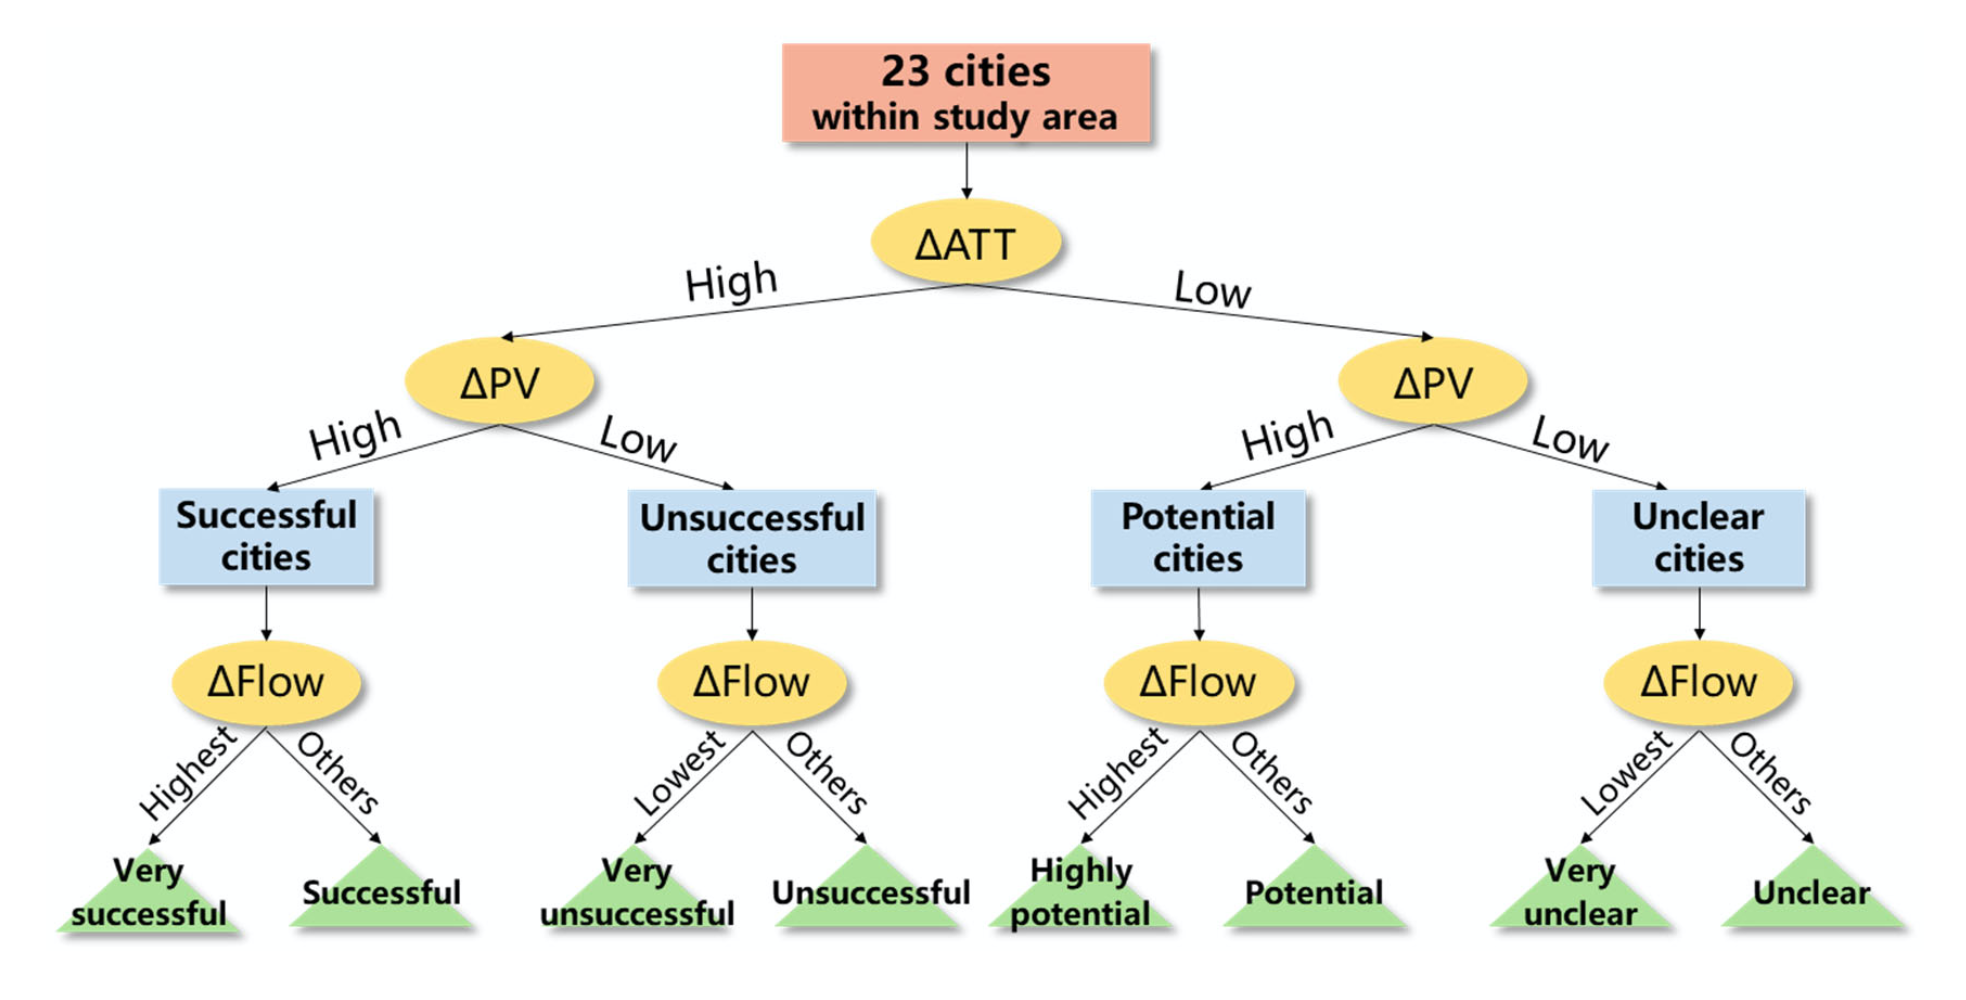
\includegraphics[width=\linewidth]{figures/binarytree_classif.png}
% rq: should have switched flow and pv - more general? ~ similar
% ! quantify impact of delta time on land use in some sense
% quite smart - planner view! - importance of thematic aspect

}


\sframe{Detailed research workflow}{

\centering
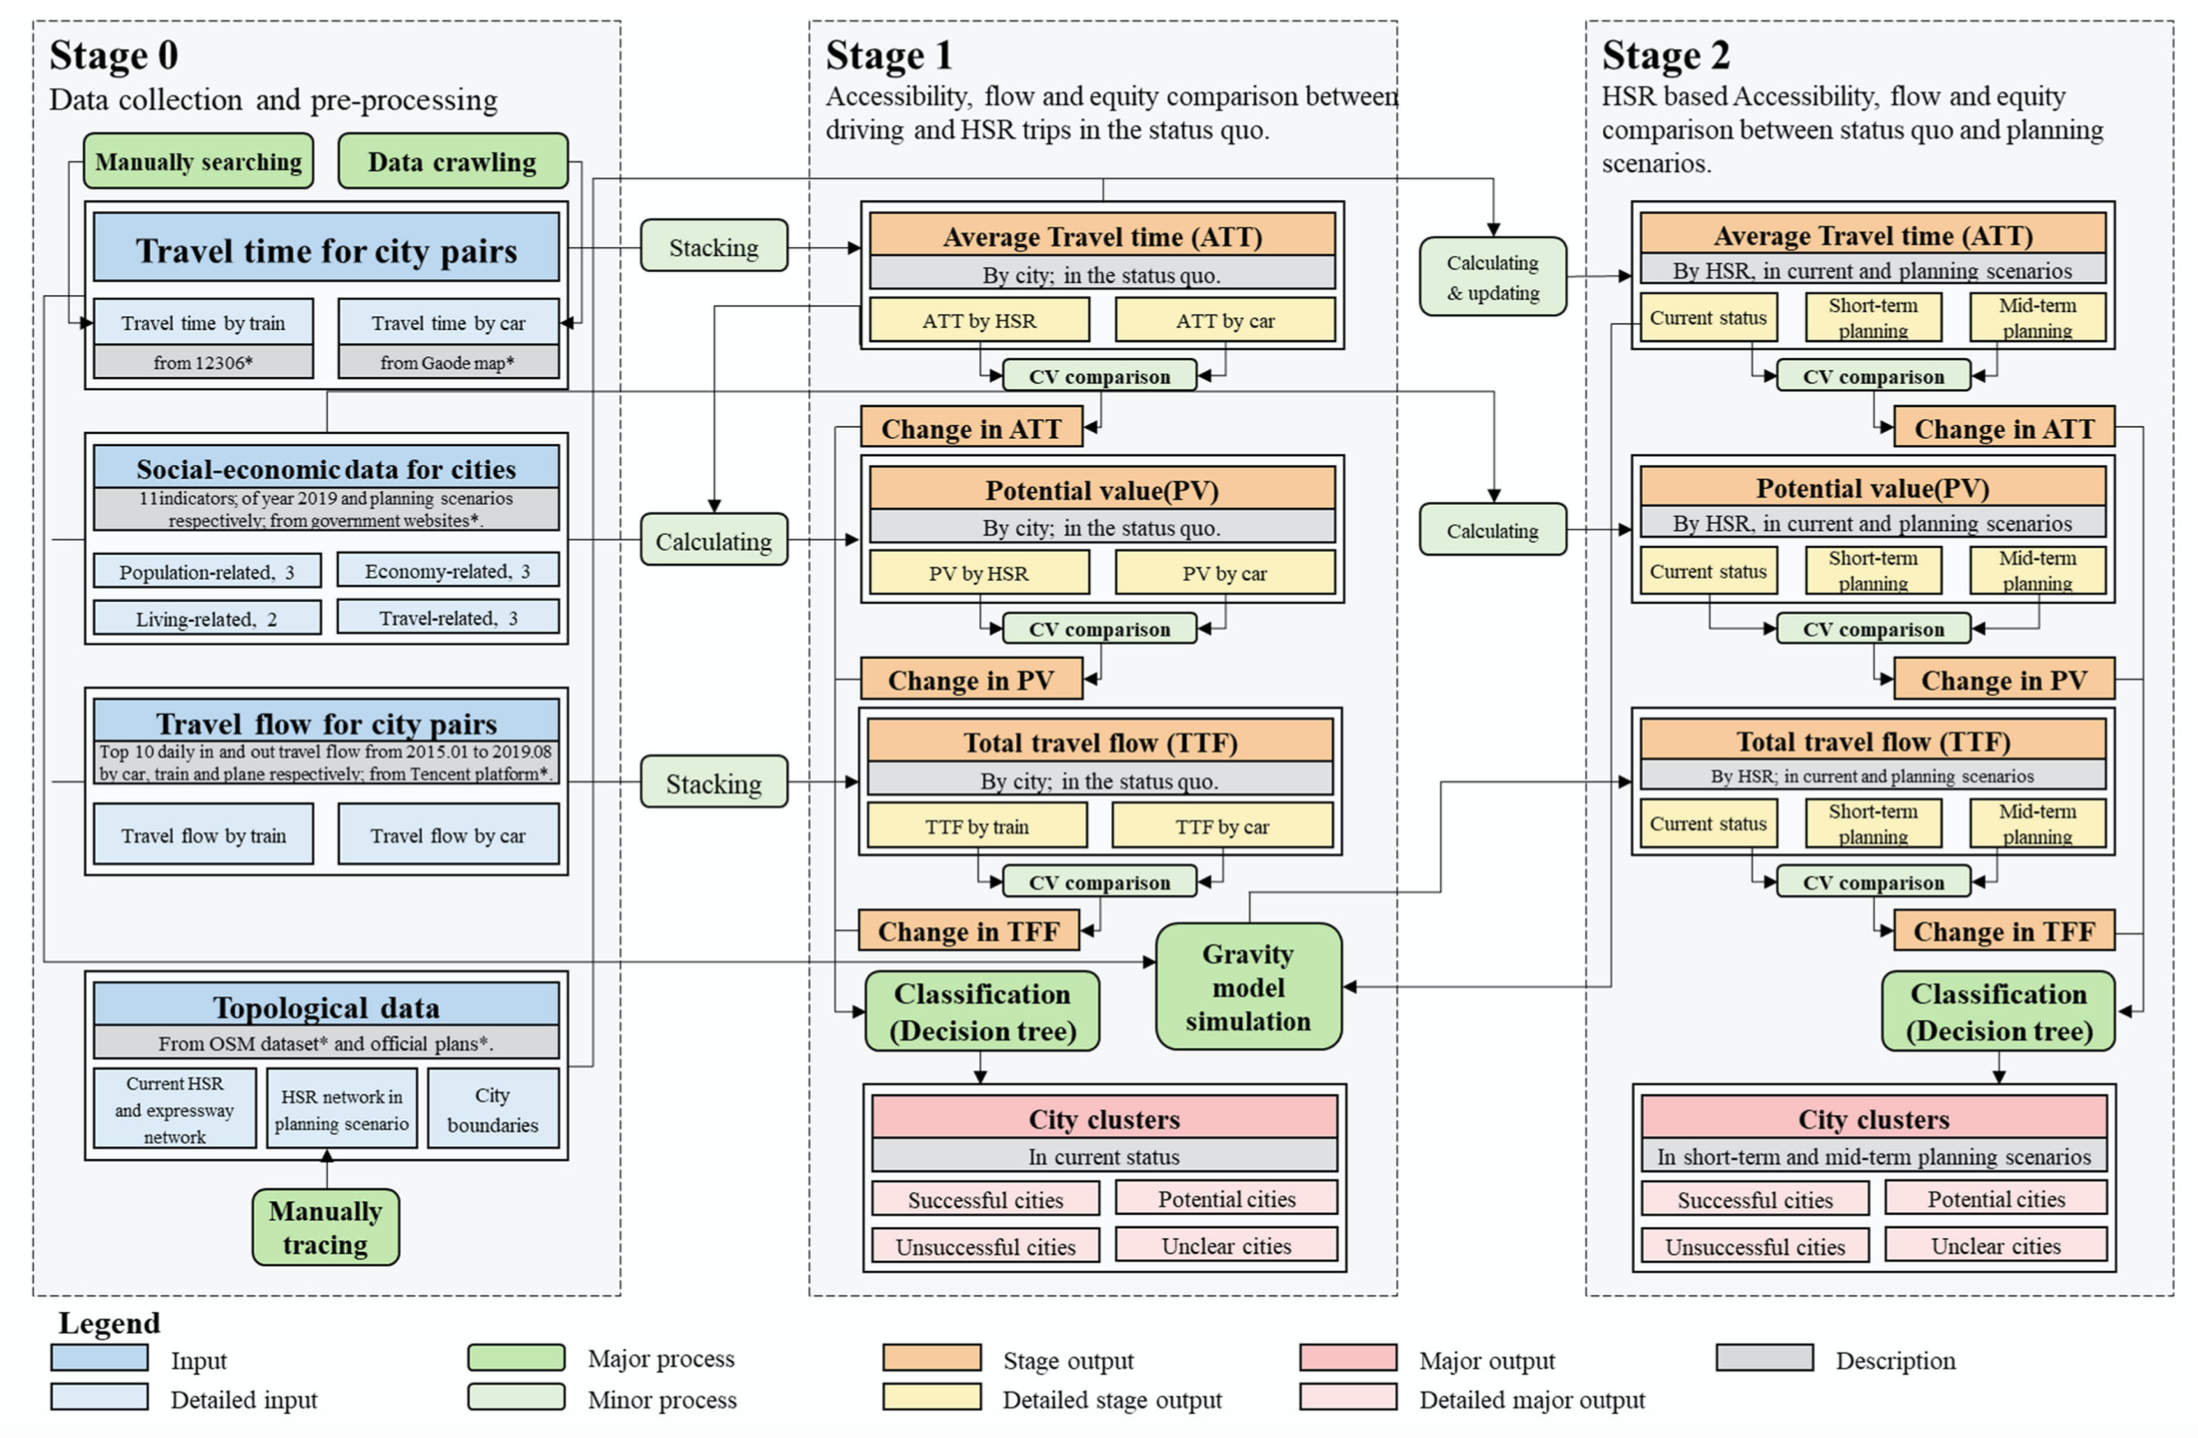
\includegraphics[width=\linewidth]{figures/research_workflow.png}

}



\section{Results}


\sframe{Travel time improvements}{

% We find that HSR considerably improved accessibility in most cities with average inter-city travel time reduced from 210 min to 168 min.

\begin{center}
	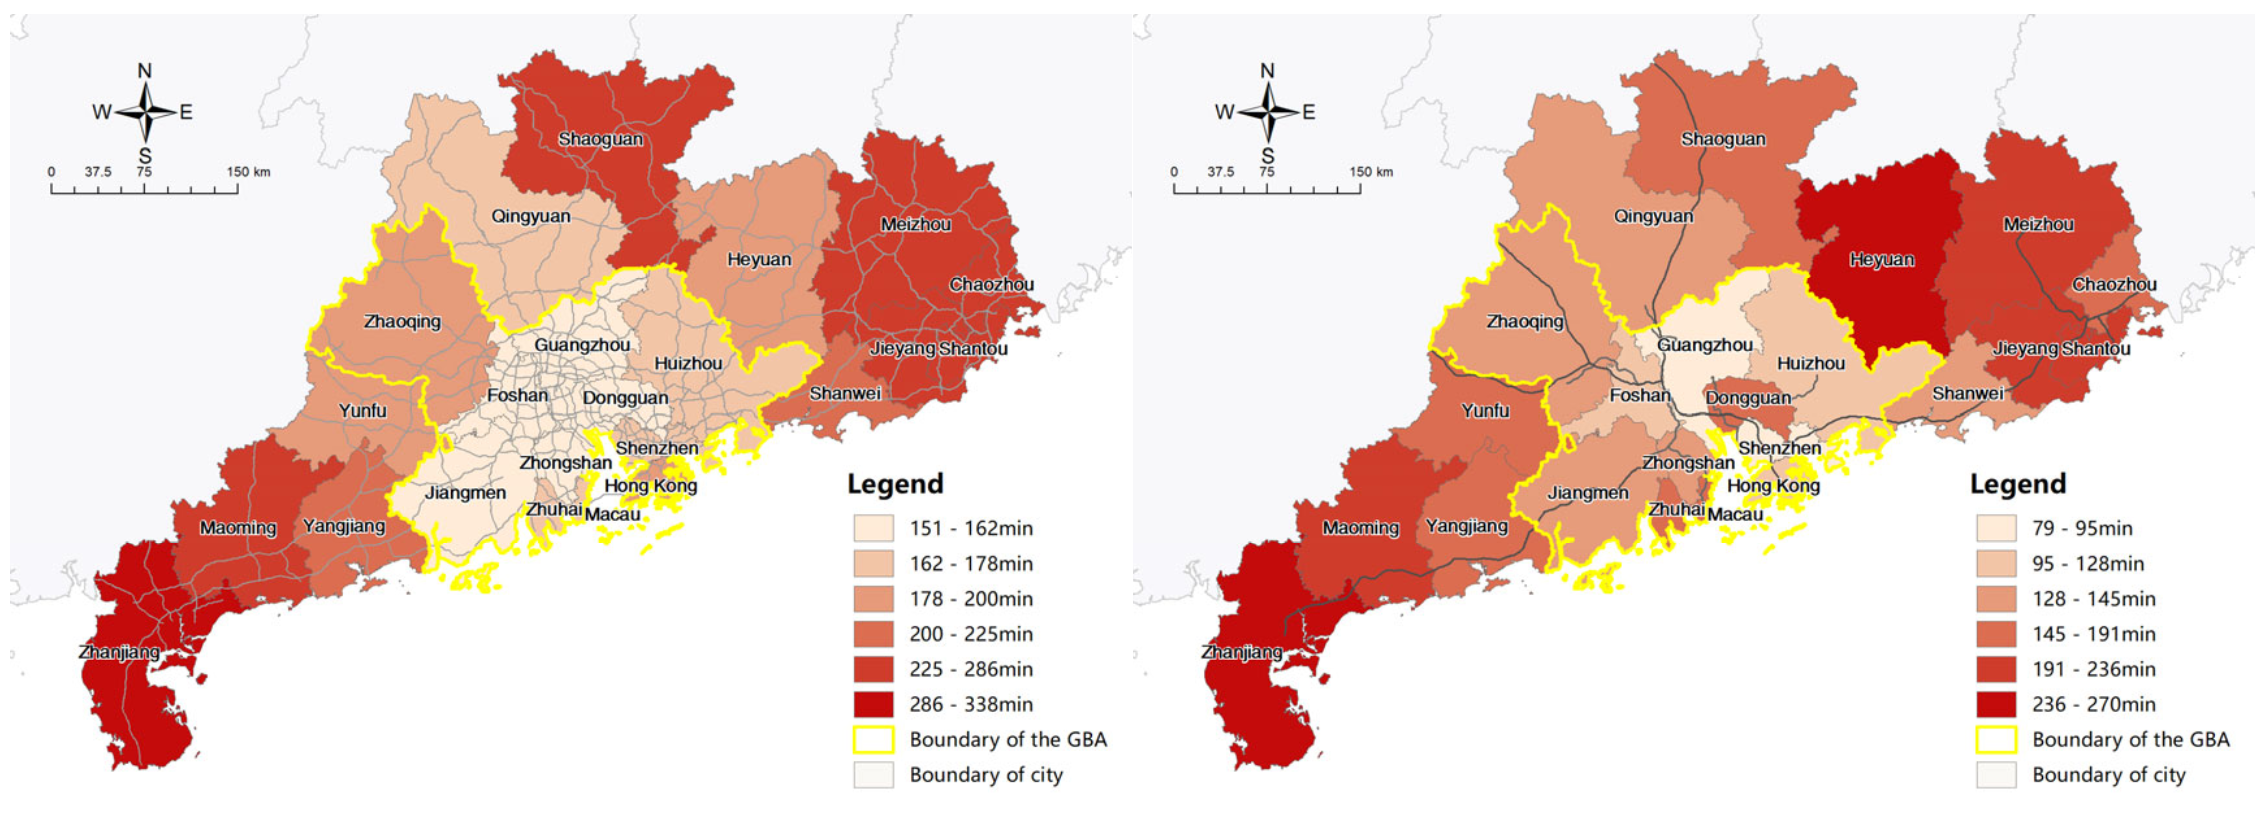
\includegraphics[width=\linewidth]{figures/ATT_map.png}
\end{center}

\textit{ATT by car (left) and HSR (right)}


}

\sframe{Increased access inequalities}{

% This first development however increased polarisation around main corridors and increased access inequality.

\begin{center}
	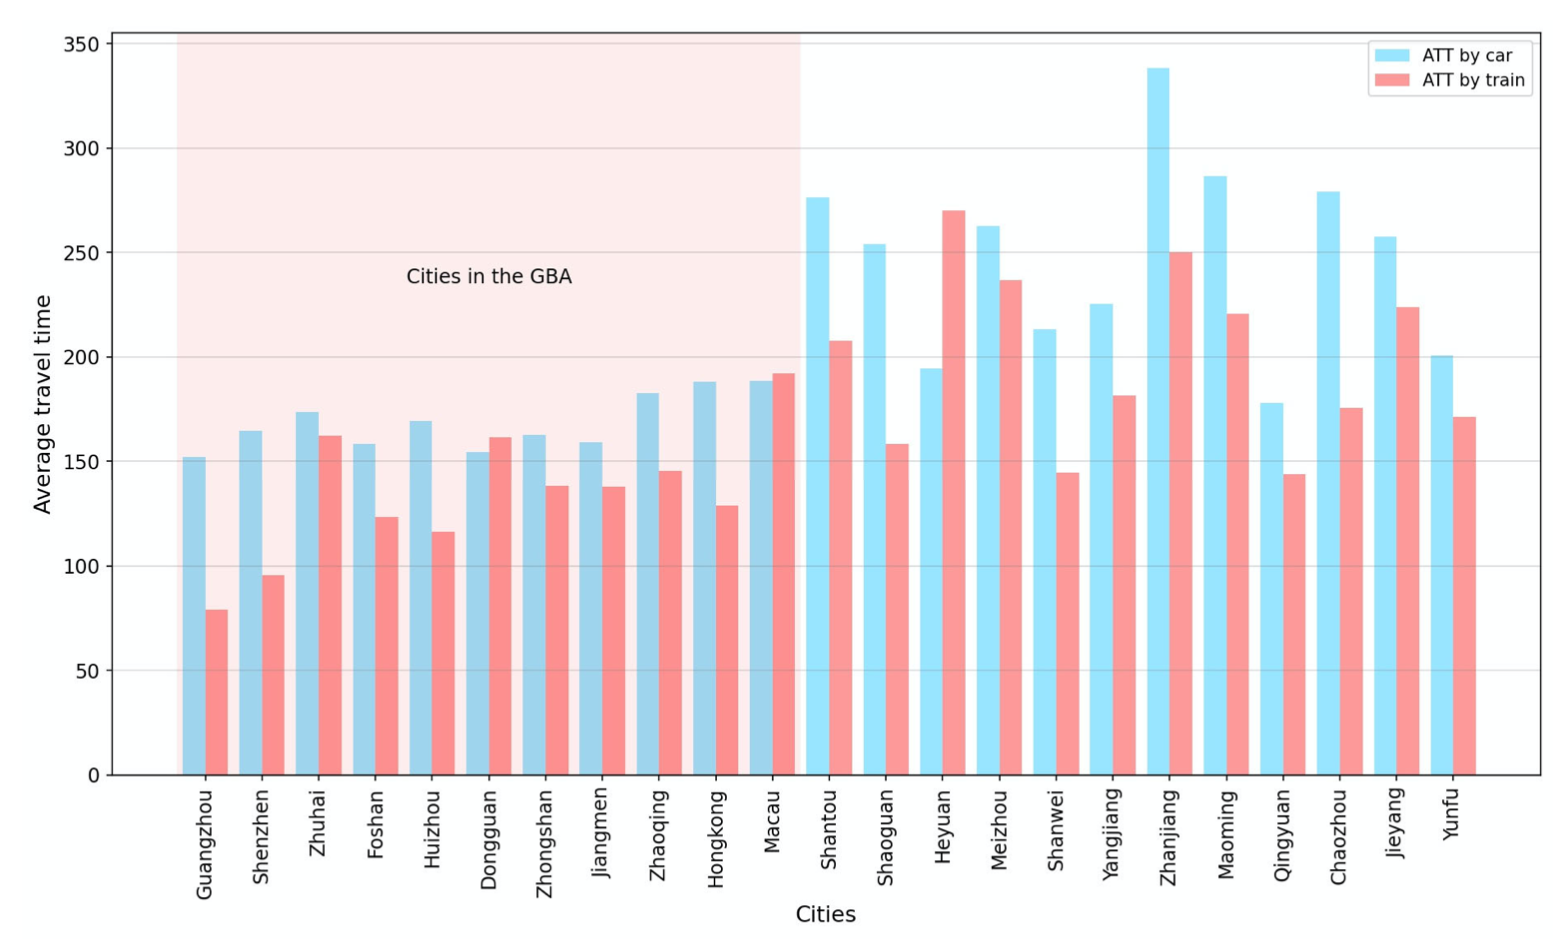
\includegraphics[width=0.75\linewidth]{figures/ATT.png}
\end{center}

\medskip

\begin{itemize}
   \item Increase in CV in GBA from 7.81\% to 23.50\%; 25.08\% to 29.26\% in Guangdong: increased access inequality
	\item Similar results with potential and travel flows
\end{itemize}


}


\sframe{City classification}{

\begin{center}
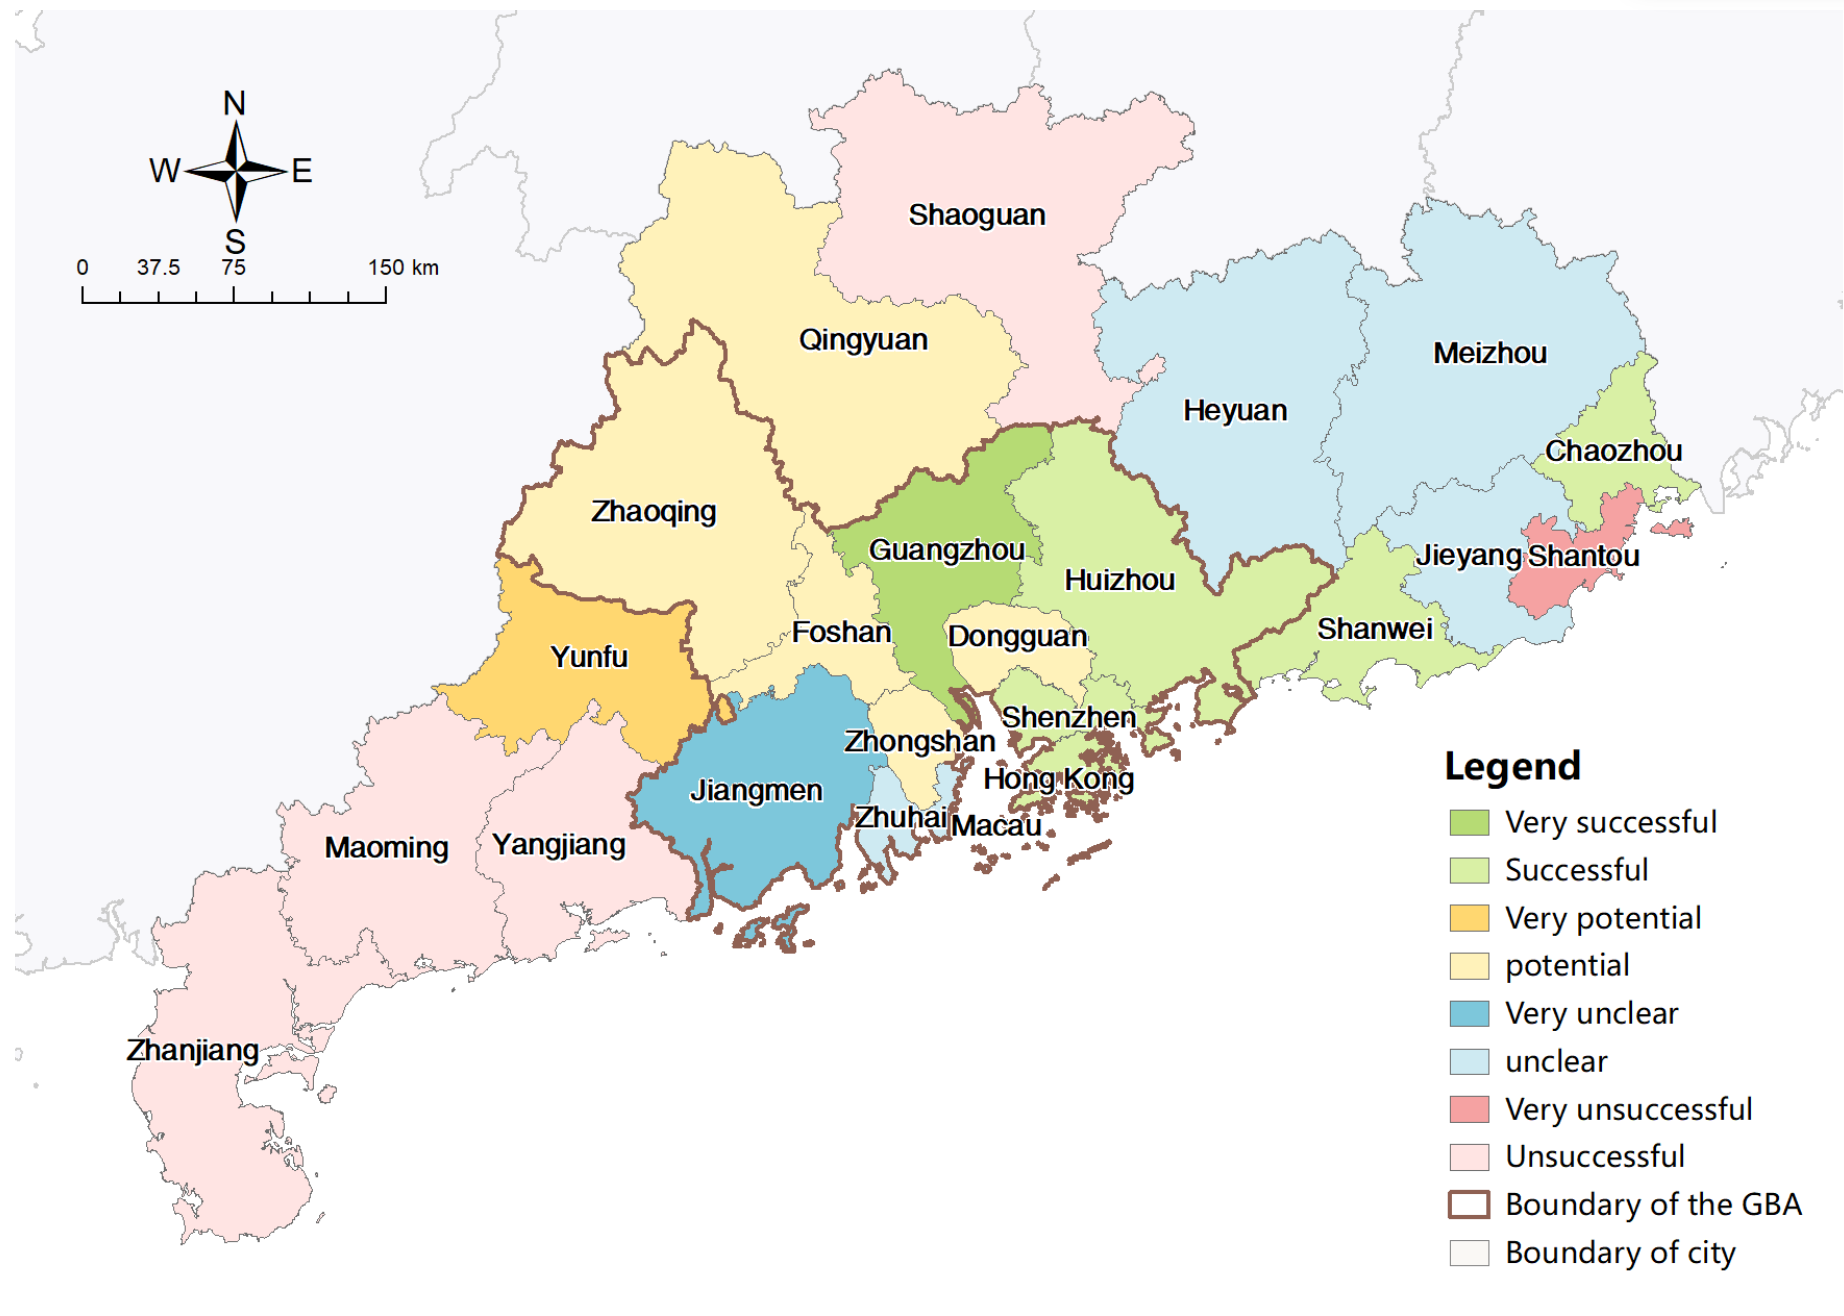
\includegraphics[width=0.75\linewidth]{figures/cityclassif.png}
\end{center}

\medskip

\textbf{Synthesis:} consequent improvements in accessibility, but increase in access inequity; centre-periphery pattern
% rq: // keynote Mike - power of centrality; rq: classif strange: correlation between indicators.


}


\sframe{Impact of new lines}{

% The mid-to-long term railway plan significantly flattens access differences and provides in particular a rebalancing between East and West of the region.

\begin{center}
	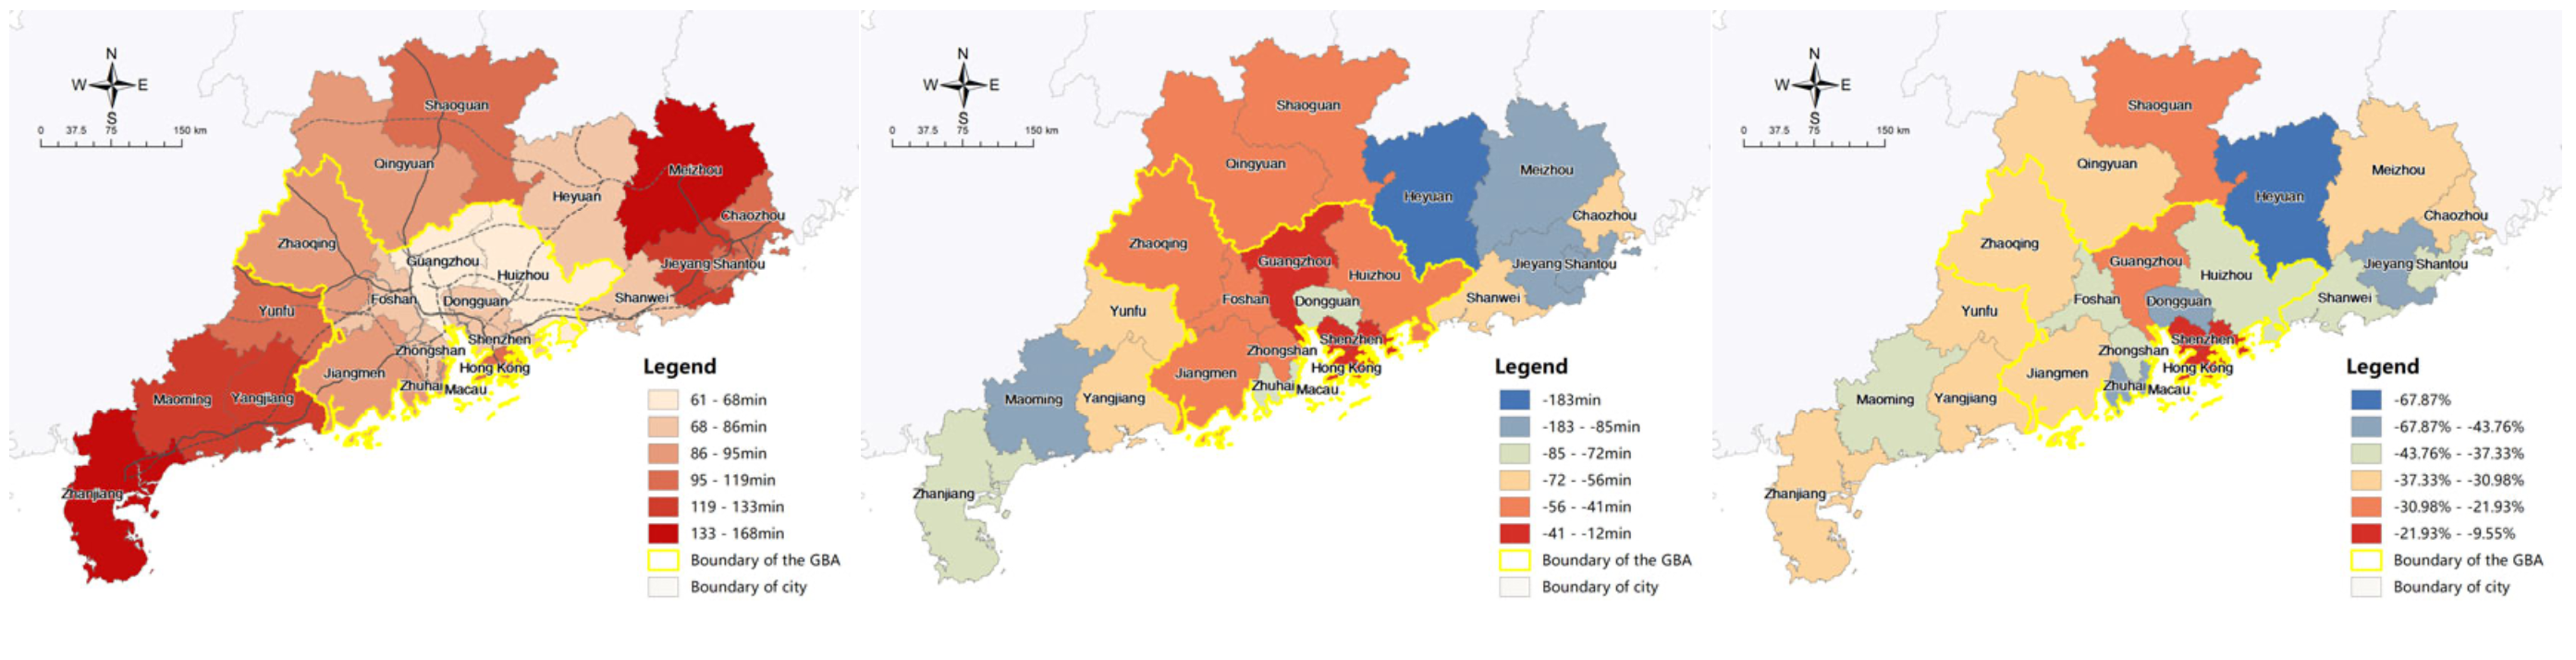
\includegraphics[width=0.9\linewidth]{figures/ATT_shortterm.png}\\
	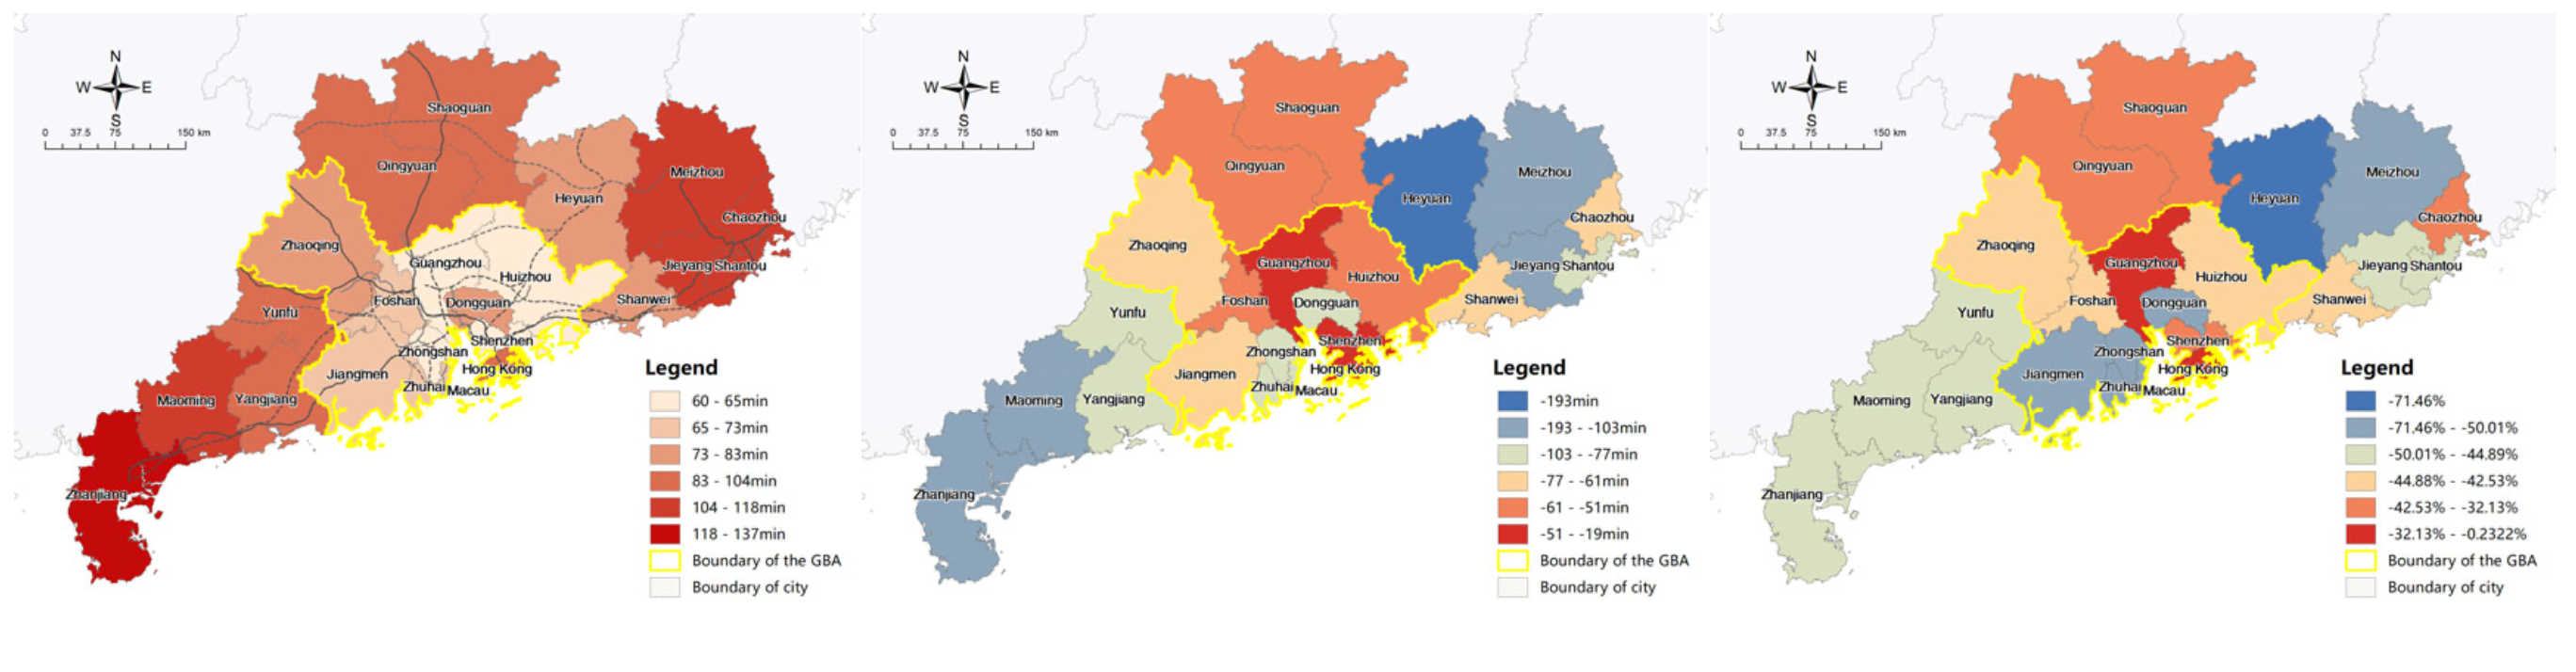
\includegraphics[width=0.9\linewidth]{figures/ATT_midterm.png}
\end{center}

\footnotesize
\textit{ATT improvements for short term (top) and middle term (bottom) scenarios}

\medskip

Rebalancing and decrease in inequality; similar results for potential and simulated flows

}


\section{Discussion}


\sframe{Discussion}{

% This evolution can be understood as an example of transport network maturation at multiple spatial and temporal scales, and suggests a need for future research to understand the interplay between governance processes at different scales and the land-use transport interaction system.

% Limitations
% spatial resolution: new fine grain data?
% no multimodal access (although detailed timetables)
% only geo access (no socioeco)

\justify

\textbf{Possible extensions}

\smallskip

$\rightarrow$ spatial resolution: new mobility data

\medskip

$\rightarrow$ multi-modal accessibility

\medskip

$\rightarrow$ accessibility and socio-economic categories

\bigskip

\textbf{Planning and theoretical implications}

\smallskip

% issue of differentiated network development; socio-economic incentives to realise

$\rightarrow$ issue of differentiated network development - compromise between spatial and temporal scales and levels of the urban hierarchy

\medskip

$\rightarrow$ role of incentives and policies to foster the impact of access improvement on land-use: co-evolution \cite{raimbault2021modeling}

\medskip

$\rightarrow$ simulation models to better understand the interplay between governance and the land-use transport interaction system across scales, in particular within MCRs \cite{raimbault2021introducing}


}



\sframe{Conclusion}{


\justify

$\rightarrow$ A study of HSR and transport equity in the GBA, using detailed train timetables

\medskip

$\rightarrow$ Immediate impacts of HSR increase access inequalities, which are decreased by future plans

\medskip

$\rightarrow$ Implication for planning and policies: compromise between short and long term effects and between scales, interactions between transportation and land-use

\bigskip
\bigskip



\textbf{Open repository}


\url{https://github.com/lizhiyuan913/Traffic_Equity_in_the_GBA} 




}






%%%%%%%%%%%%%%%%%%%%%
\begin{frame}[allowframebreaks]
\frametitle{References}
\bibliographystyle{apalike}
\bibliography{biblio}
\end{frame}
%%%%%%%%%%%%%%%%%%%%%%%%%%%%










\end{document}





